%!TEX root = ../../Master.tex
\section{Laudon \& Laudon Modellen}
Denne rapport er opbygget ud fra Laudon \& Laudon modellen~\cite{laudon}. Denne model er designet til at analysere et informationssystem, med henblik på at lave et produkt. Et informationssystem er beskrevet i~\cite{laudon2006management}: \enquote{Et informationssystem kan teknisk defineres som en mængde af sammenhørende komponenter. Disse komponenter indsamler (eller henter), processerer, gemmer og distribuerer information til at hjælpe med beslutningstagen, koordination og kontrol i en organisation. Udover dette, kan informationssystemet også hjælpe bestyrere og ansatte til at analysere problemer, visualisere komplekse emner og kreere nye produkter.}

\begin{figure}
  \centering
  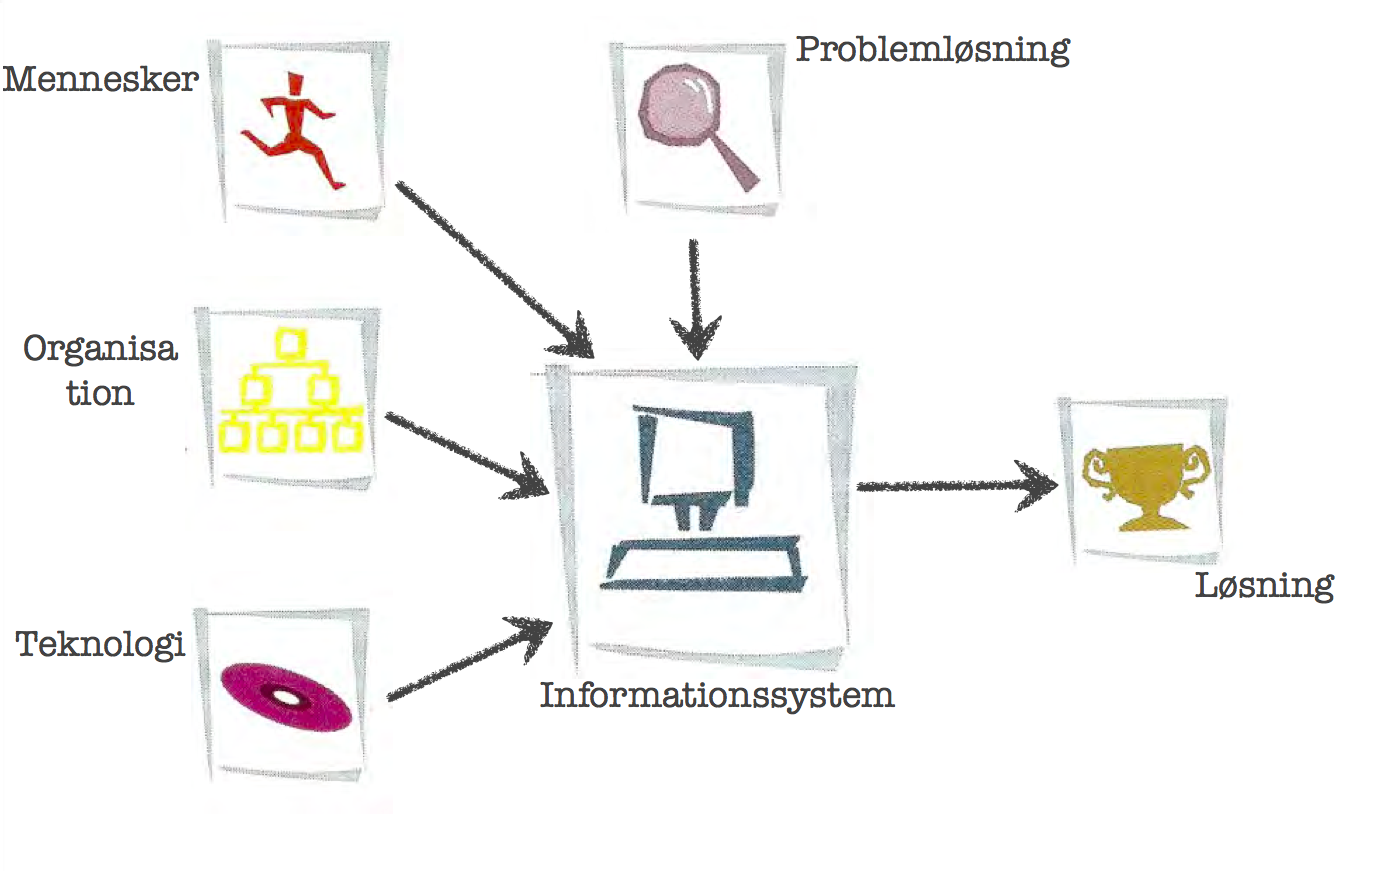
\includegraphics[width=\textwidth]{laudon}
	\caption{Oversigt over Laudon \& Laudon modellen}
	\label{fig:oversigt_laudon}
\end{figure}

I denne rapport vil informationssystemet blive omtalt som løsningen, og det der i modellen hedder løsning, er den effekt informationssystemet giver. Et overblik af modellen kan ses på \cref{fig:oversigt_laudon}. 

Modellen sørger altså for at løsningen er kontekstuel relevant i forhold til problemet. De forskellige elementer i modellen der skal undersøges, er mennesker, teknologi, organisation, problem, løsning og effekten. Modellen giver mulighed for at lave en løsning der tager udgangspunkt i virkeligheden, og derved løser de reelle krav der er til løsningen.
